% 4.1 O1 Energy and carbon. OWNER: Aditya. First draft by Aryan from the presented deck (slides 16-19) and the D2
% diagnostics (report/analysis/d2_growth_diagnostics.py). Numbers: claims.csv rows O1, O1/D2, S1/O1; claims_report.csv.
\subsection{O1: Energy and carbon}\label{sec:o1}

\paragraph{US data-centre electricity} The clearest evidence that the AI era broke the cloud-era plateau is in the US
series of the Lawrence Berkeley National Laboratory. US data centres used about 60\,TWh a year in 2014--2016, 76\,TWh in
2018 and 176\,TWh in 2023 \citep{shehabi2024}. The report gives the growth as about 7\% a year for 2014--2018 and 18\%
a year for 2018--2023, which means the doubling time fell from about 10 years to about 4. Globally, the IEA estimates
growth of about 12\% a year since 2017 \citep{iea2025}; that is a different series, so we do not splice it in.

\begin{table*}[t]\centering
\caption{Growth on one scale (deliverable D2). $r$: annual growth rate; $T_2$: doubling time. Intervals (95\%) for
$T_2$ only where a yearly series exists: OLS, and Newey--West (HAC), which allows for serial correlation in the
residuals. Data-centre rows rest on two published values each, so they have no interval. The US rates are approximate,
as stated by LBNL. The world 2024--2030 row is a projection (IEA base case: 415 to 945\,TWh).}
\label{tab:growth}
\footnotesize\renewcommand{\arraystretch}{1.1}\setlength{\tabcolsep}{4.2pt}
\begin{tabular}{@{}P{1.95cm} P{3.0cm} l r r c c c P{2.4cm}@{}}
\toprule
Phase & Series & Period & $r$ (\%/yr) & $T_2$ (yr) & 95\% CI, OLS & 95\% CI, HAC & $R^2$ & Basis \\
\midrule
\tabin{tables/growth.tex}
\bottomrule
\end{tabular}
\end{table*}

\paragraph{Three phases on one scale} \Tab{tab:growth} puts every series on the same scale. In the Great Acceleration,
world primary energy grew by 2.4\% a year and doubled about every 30 years. In the cloud era it slowed to 1.2\% a year,
and world data-centre electricity barely moved: the +6\% of 2010--2018 is 0.7\% a year, a doubling time of about 95
years. In the AI era, US data-centre electricity doubles about every four years, and the IEA's projection for the world
implies 14.7\% a year to 2030. The driver sits in the last row: the training compute of notable AI models has grown by
about 330\% a year since 2010, doubling roughly every six months.

\paragraph{Why the plateau ended} Two series explain the gap between compute and electricity. US
AI-accelerated servers used under 2\,TWh in 2017 and over 40\,TWh in 2023 \citep{shehabi2024}. Over the same period
the main efficiency lever of the cloud era stopped working: the average PUE of data centres fell from 2.50 in 2007 to
1.65 in 2014, then stayed near 1.5 (1.54 in 2025) \citep{uptime2025}. The one-off gains of better cooling and moving
work into large hyperscale sites were used up, so growth in computing began to show up as growth in electricity. PUE
measures the building's overhead, not the chips; we did not test performance per watt.

\begin{finding}{Finding 1. Compute broke upward in 2011; electricity followed only around 2018}
The breakpoint test puts the acceleration of AI compute in 2011 (doubling time 1.7 to 0.5 years). Data-centre
electricity rose only 6\% in 2010--2018, and in the US its growth jumped from about 7\% to 18\% a year after 2018, when
AI servers' demand rose more than twenty-fold and PUE had been flat since 2014. The efficiency story is \emph{partly
supported}: the building-efficiency half fits; the chip-efficiency half was not tested.
\end{finding}

\begin{figure}[t]\centering
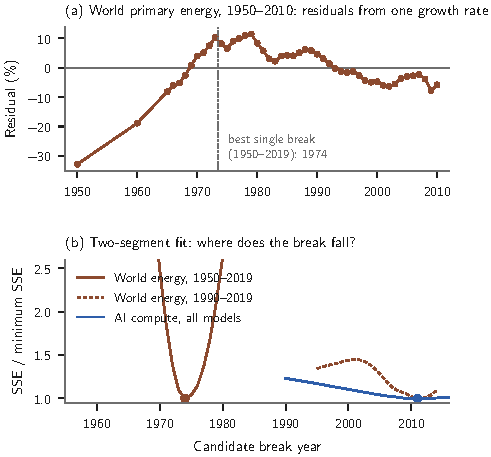
\includegraphics[width=\linewidth]{figs/d2_diagnostics.pdf}
\caption{Fit diagnostics for the growth table. (a) Residuals of world energy around a single 1950--2010 growth rate:
long runs of the same sign (Durbin--Watson 0.15), so the OLS interval is too narrow. (b) Two-segment fits: residual sum
of squares for each candidate break year, relative to the best. World energy breaks in 1974 over 1950--2019, but in
2011 over 1990--2019; AI compute breaks in 2011.}
\label{fig:d2}
\end{figure}

\begin{table}[t]\centering
\caption{Breakpoint tests (two-segment fits). $\Delta$BIC $<0$ favours a break; the more negative, the stronger.}
\label{tab:breaks}
\footnotesize\renewcommand{\arraystretch}{1.1}\setlength{\tabcolsep}{3.6pt}
\begin{tabular}{@{}l l r r l r@{}}
\toprule
Series & Window & $n$ & Break & Before $\to$ after & $\Delta$BIC \\
\midrule
\tabin{tables/breaks.tex}
\bottomrule
\end{tabular}
\end{table}

\paragraph{How far the fits can be trusted (D2 diagnostics)} \Fig{fig:d2} and \Tab{tab:breaks} check the fits behind
\Tab{tab:growth}. Three points stand out. First, the Great Acceleration fit is good ($R^2=0.95$), but its residuals are
strongly autocorrelated (Durbin--Watson 0.15, lag-one correlation 0.93): world energy ran above trend from about 1970 to
the early 1990s and below it after the mid-1990s. The point estimate of 30 years does not change, but an honest interval is 25.6--35.7 years
rather than 27.9--32.0. Second, the compute fit has a tight interval only because it rests on 478 models; individual
models scatter by about 1.7 orders of magnitude around the line ($R^2 = 0.66$), because the list mixes frontier and
smaller models. Third, the breaks are real but depend on the window. AI compute breaks in 2011 with very strong support
($\Delta$BIC $-245$). World energy breaks in 1974, the first oil shock, over 1950--2019 ($-147$), but in 2011 over
1990--2019, with only weak support ($-4$). The 1950 boundary itself cannot be tested, because the series is decadal
before 1965, and the data-centre rows rest on two published points each, so they allow neither an interval nor a break
test.

\begin{reading}
Our reading: the phase boundaries of 1950, 2010 and 2019 are a framing, and the data treat them that way. They support
a break in compute in 2011 and a break in data-centre electricity around 2018, not one clean boundary for everything.
\end{reading}

\begin{figure}[t]\centering
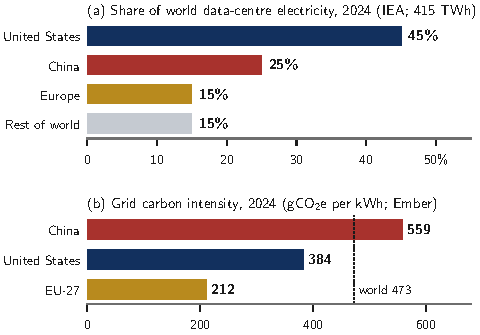
\includegraphics[width=\linewidth]{figs/o1_regional_carbon.pdf}
\caption{Where data-centre electricity is used, and how much \cotwo\ each kWh carries. (a) IEA shares of the
415\,TWh used in 2024. (b) Average grid carbon intensity in 2024 (Ember); the EU-27 stands in for the IEA's
``Europe''. These are grid averages, used as benchmarks, not data-centre emission estimates.}
\label{fig:o1}
\end{figure}

\paragraph{The load is regional; its carbon depends on the grid} Three regions use 85\% of data-centre electricity
(\Fig{fig:o1}). What that electricity emits depends on the grid that supplies it: in 2024 a kWh carried 559\,g of
\cotwo-equivalent in China, 384\,g in the United States and 212\,g in the EU, against a world average of 473\,g
\citep{ember2026}. The same kWh therefore emits about 2.6 times as much in China as in the EU. Electricity is a
regional load, felt by grids and local air; carbon is a global impact, but its size is set by where the load sits.
